\documentclass[11pt]{report}
\newcommand{\userName}{Rebecca Miko}
\newcommand{\institution}{University of Hertfordshire}

%Packages
\usepackage{graphicx}
\usepackage{xr}
\usepackage{hyperref}
\usepackage{geometry}

\geometry{margin=1in}



% Begin document
\begin{document}

\pagenumbering{arabic}
\begin{center}
{\Huge Progress Report}
\end{center}
\section*{Abstract}
The olfactory bulb in mammals is responsible for receiving, processing and relaying olfactory information (odours). This project investigates how naturalistic temporally fluctuating odour signals are processed and which neurons or neural mechanisms are able to extract information from these signals. Multiple computation models were created to represent different OB circuits between periglomerular cells and mitral cells using NEURON (Hines and Carnevale, 2006, 2001). The results show that the strength and frequency of these odour signals can be determined by looking at a combination of the latency and the firing rates of the output from the mitral cells. 

\section*{Research question:}
Can we predict the strength and frequency of the input by looking at two features: Firing Rates and Latency?\\

\begin{figure}[!ht]
\centering
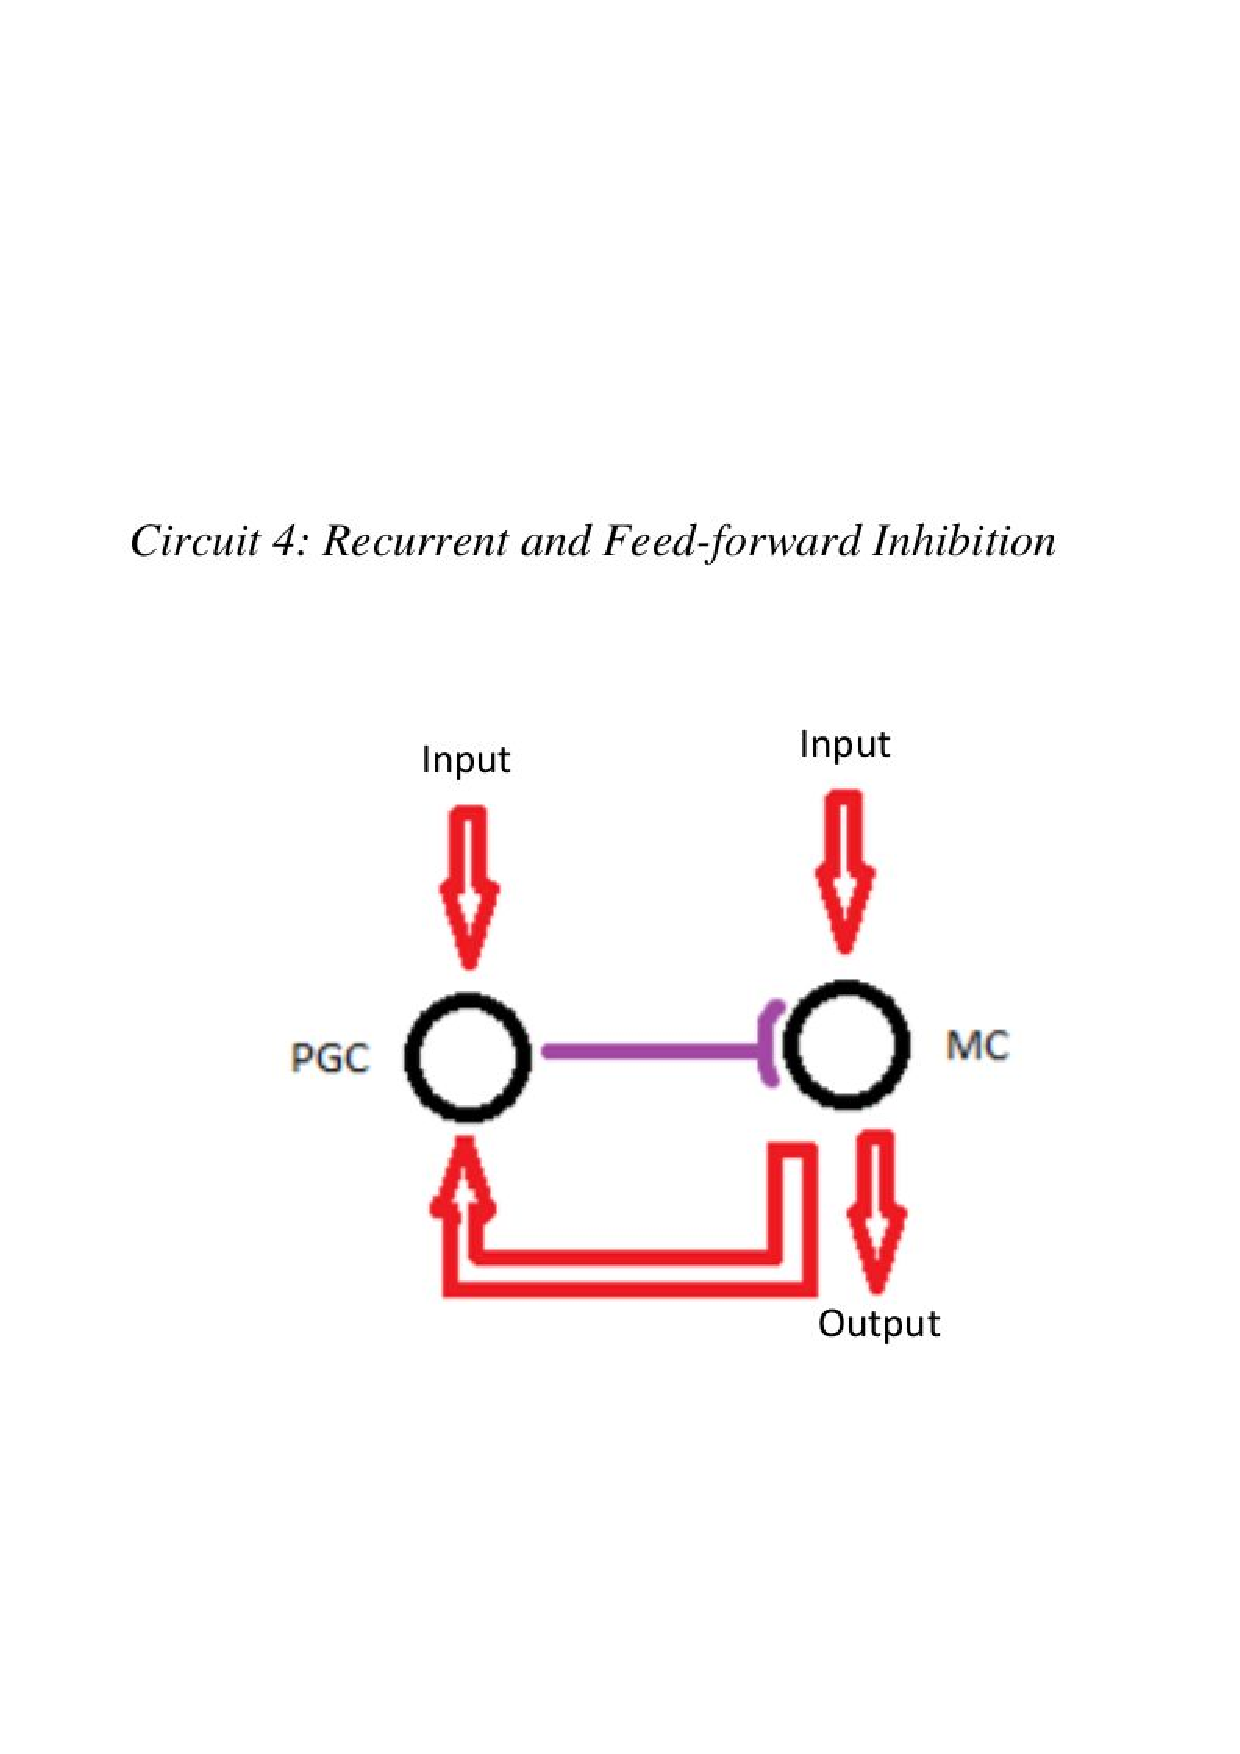
\includegraphics[trim={0 6cm 0 8cm},clip, scale=0.5]{Analysis-6-11-17/Circuit_4.pdf}
\caption{showing the full model.}
\end{figure} 

Figure 1 shows the full model (denoted as circuit 4). The PGC (periglomerular cell) and the MC (mitral cell) both recieve input, both the feed-forward and recurrent inhibition is considered, and the output from the MC is analysed. 
\newpage

\begin{figure}[!ht]
\centering
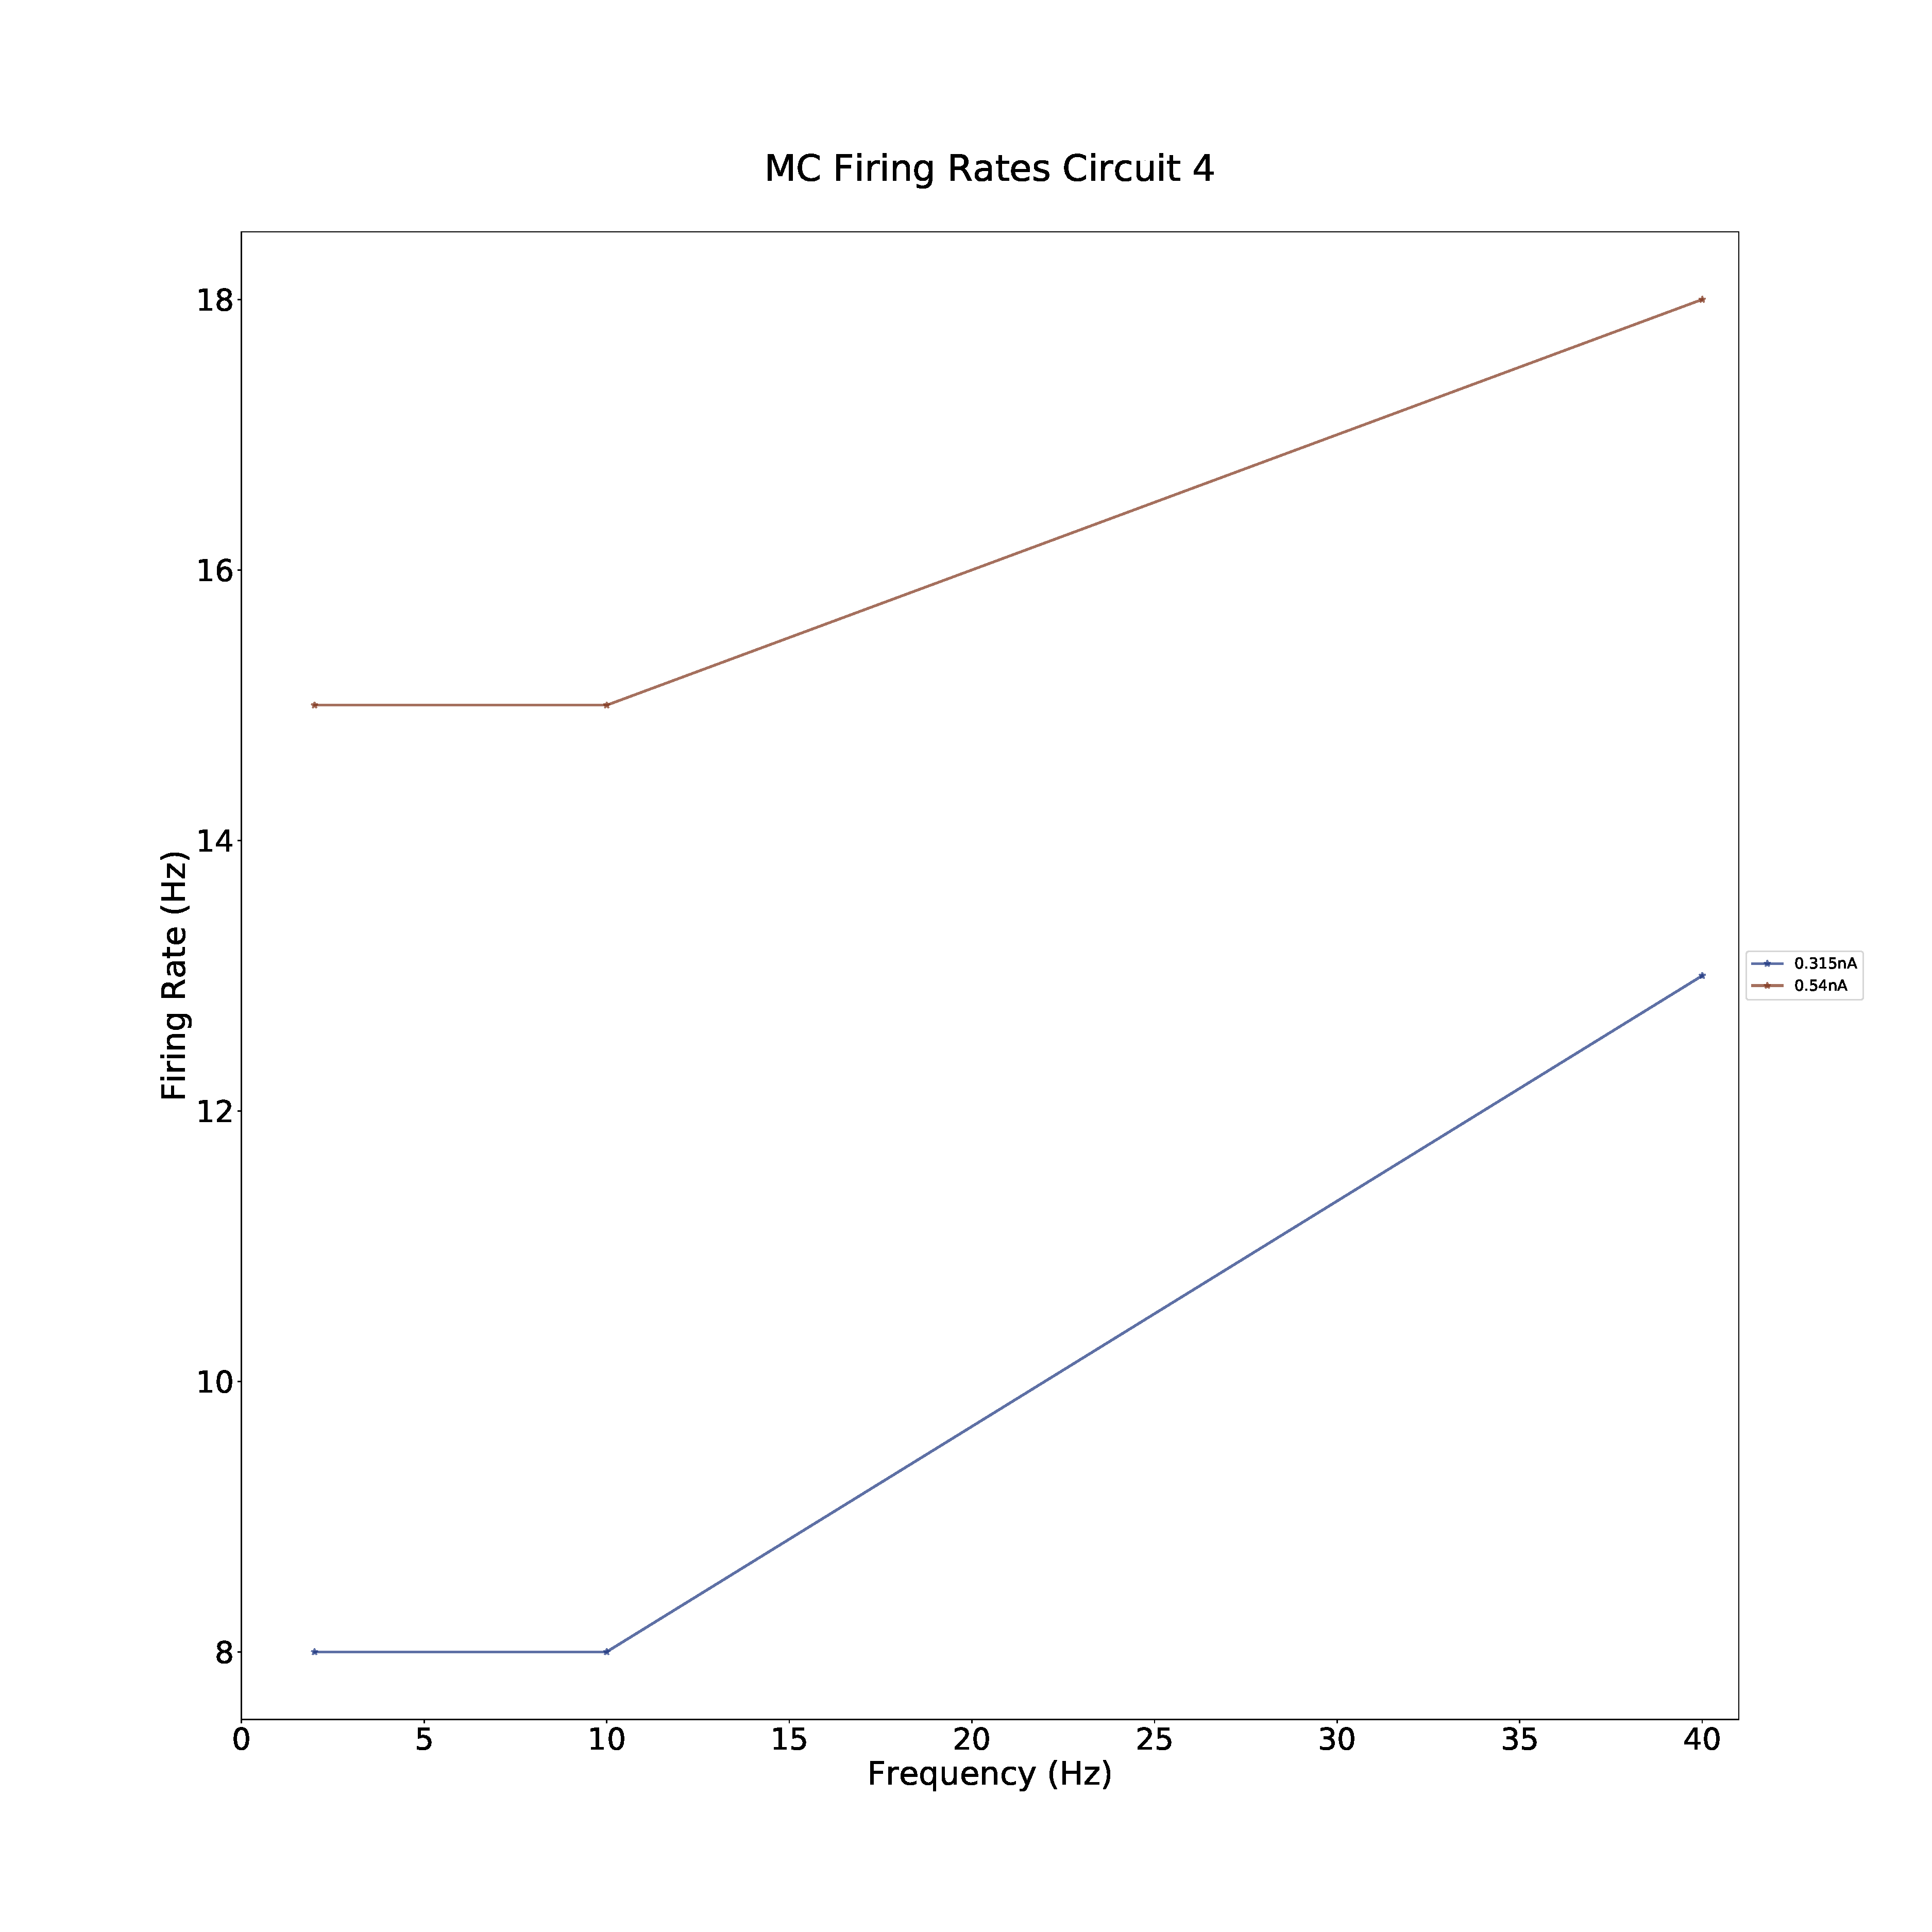
\includegraphics[scale=0.3]{Analysis-6-11-17/MC_firing_rate_C4.pdf}
\caption{showing the mitral cell firing rates for circuit 4.}
\end{figure} 

In figure 2, it is clear that the firing rates can be used to determine the strength of the input current. However, the frequency of the input current is still unclear. 
\newpage

\begin{figure}[!ht]
\centering
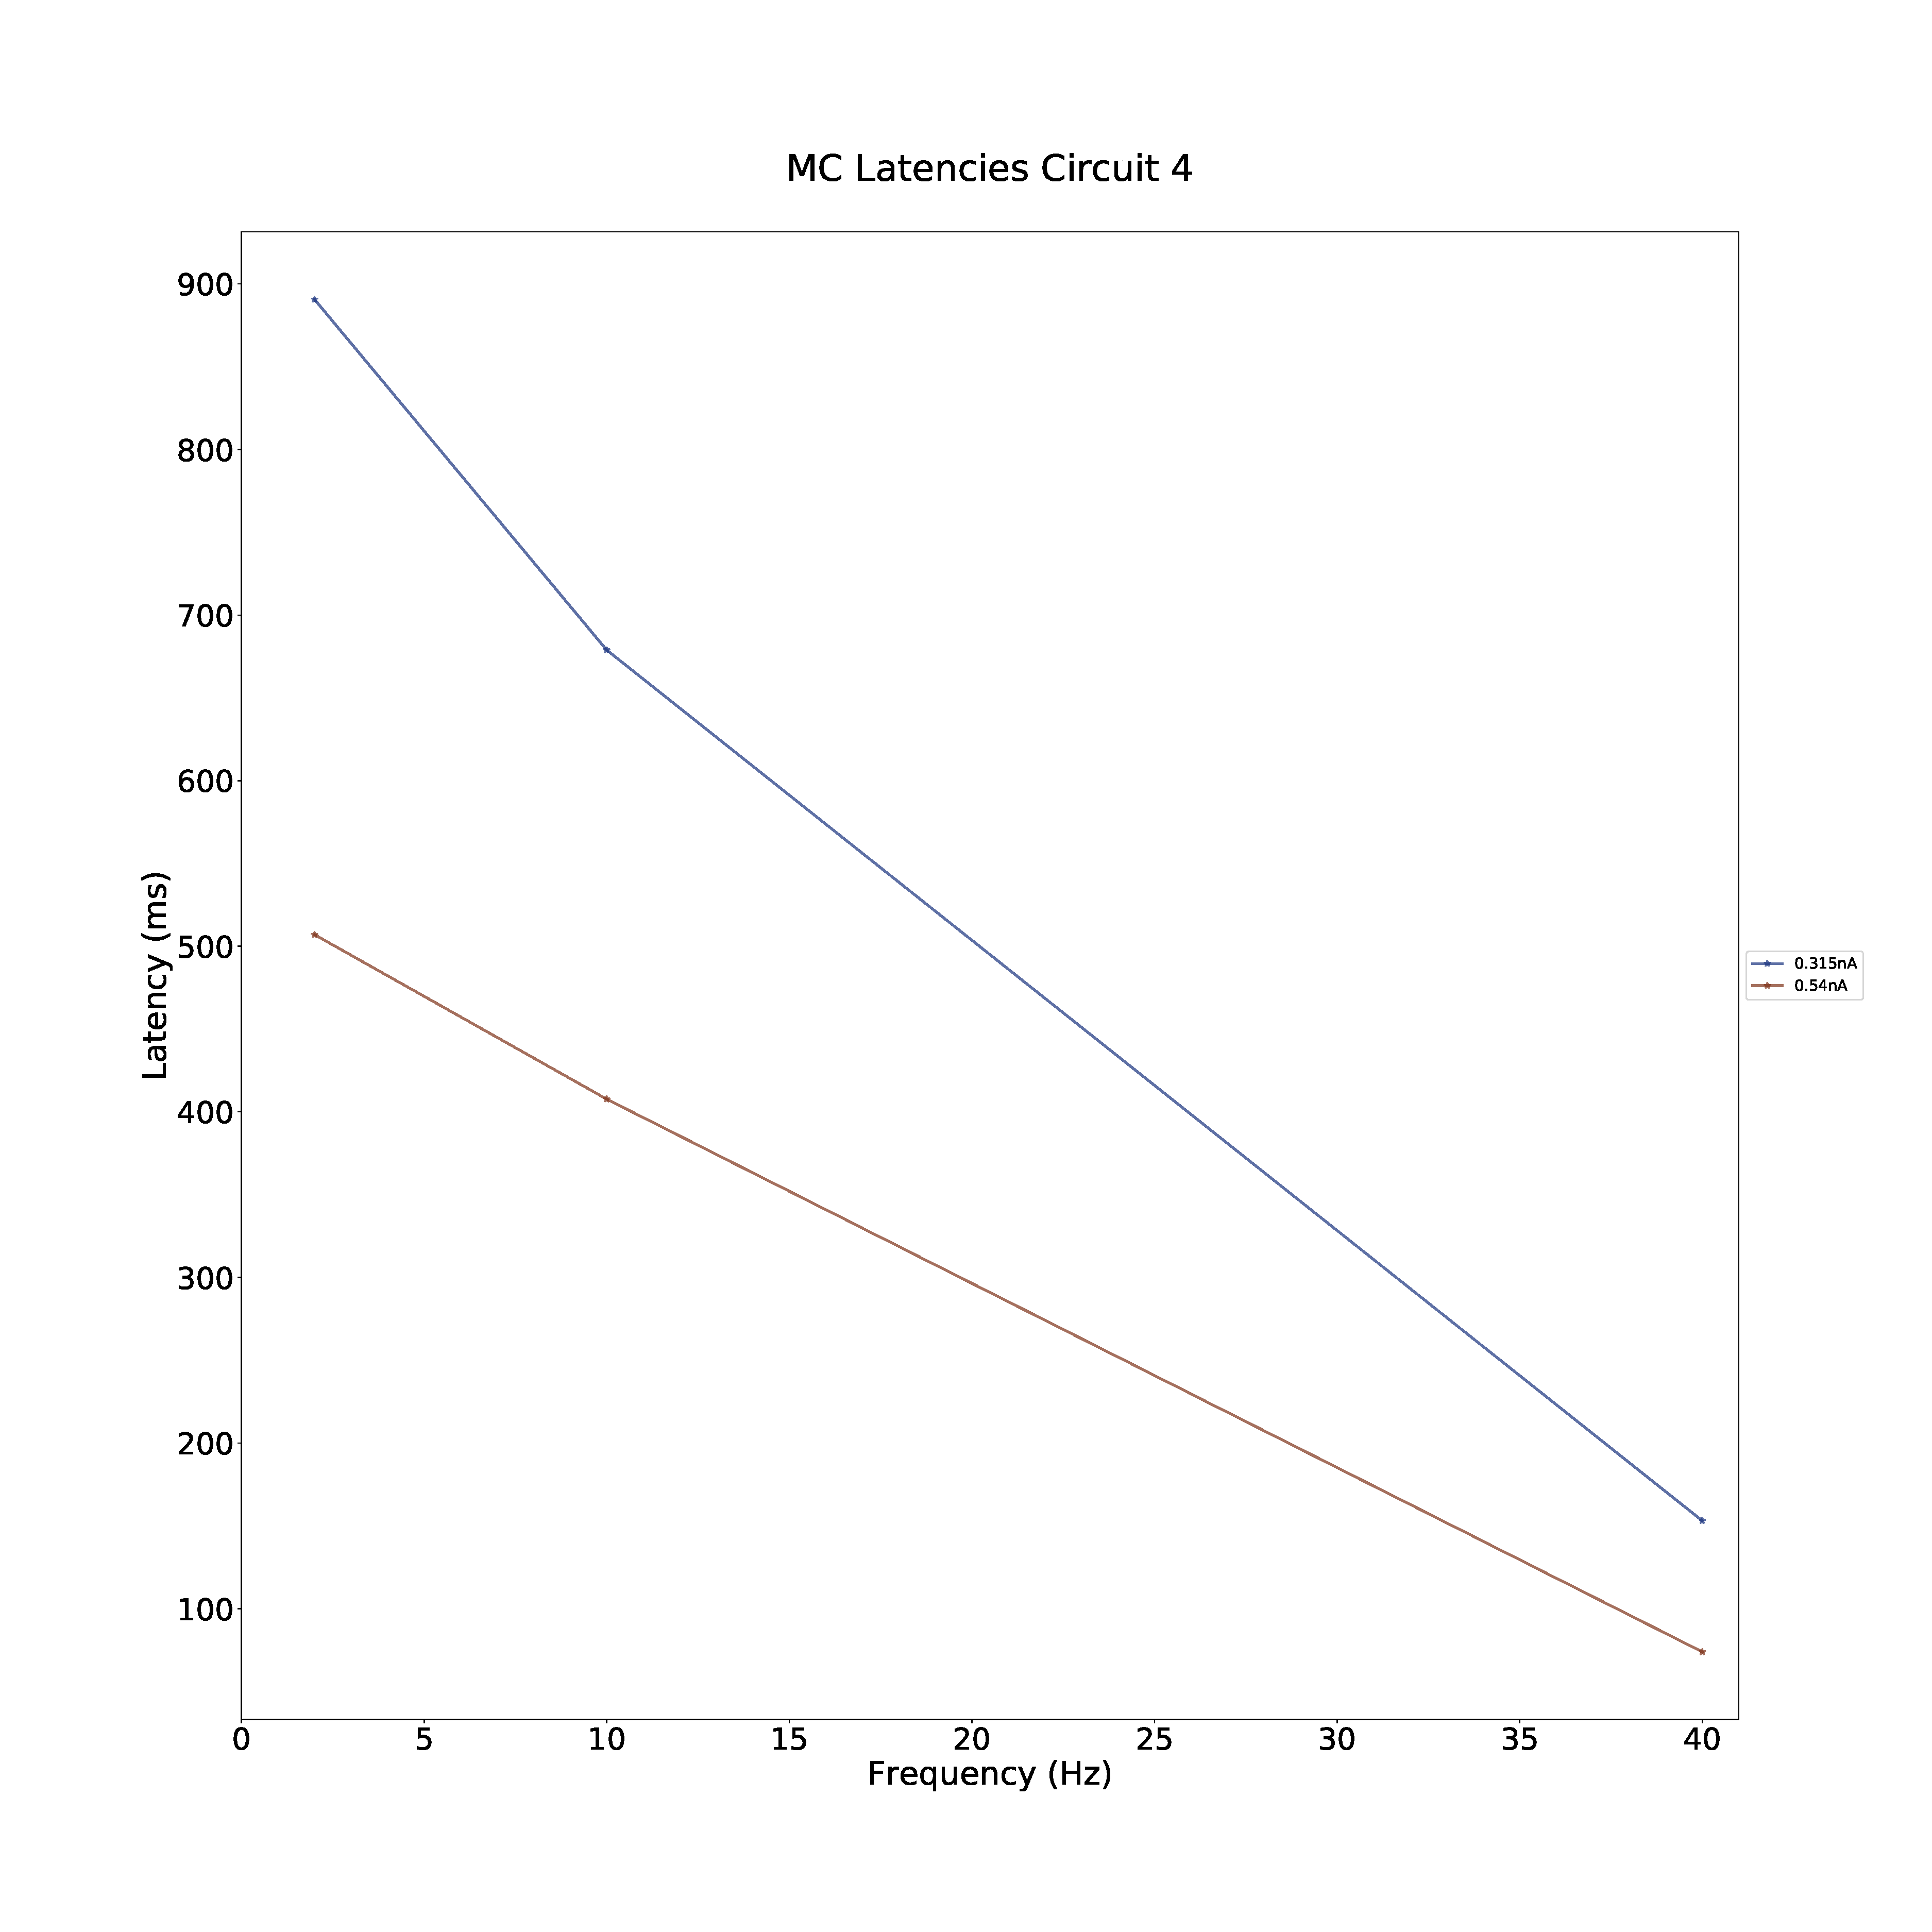
\includegraphics[scale=0.3]{Analysis-6-11-17/MC_latencies_C4.pdf}
\caption{showing the mitral cell latencies for circuit 4.}
\end{figure} 

Figure 3 shows that we can determine the frequency of the input from the latencies. Therefore, we can predict the strength and frequency of the input by looking at a combination of both firing rates and latency.

\section*{New research question:}
The strength and frequency of the input can be predicted by looking at the firing rates and latency, as described above. What mechanism is responsible for these results?

\begin{figure}[!ht]
\centering
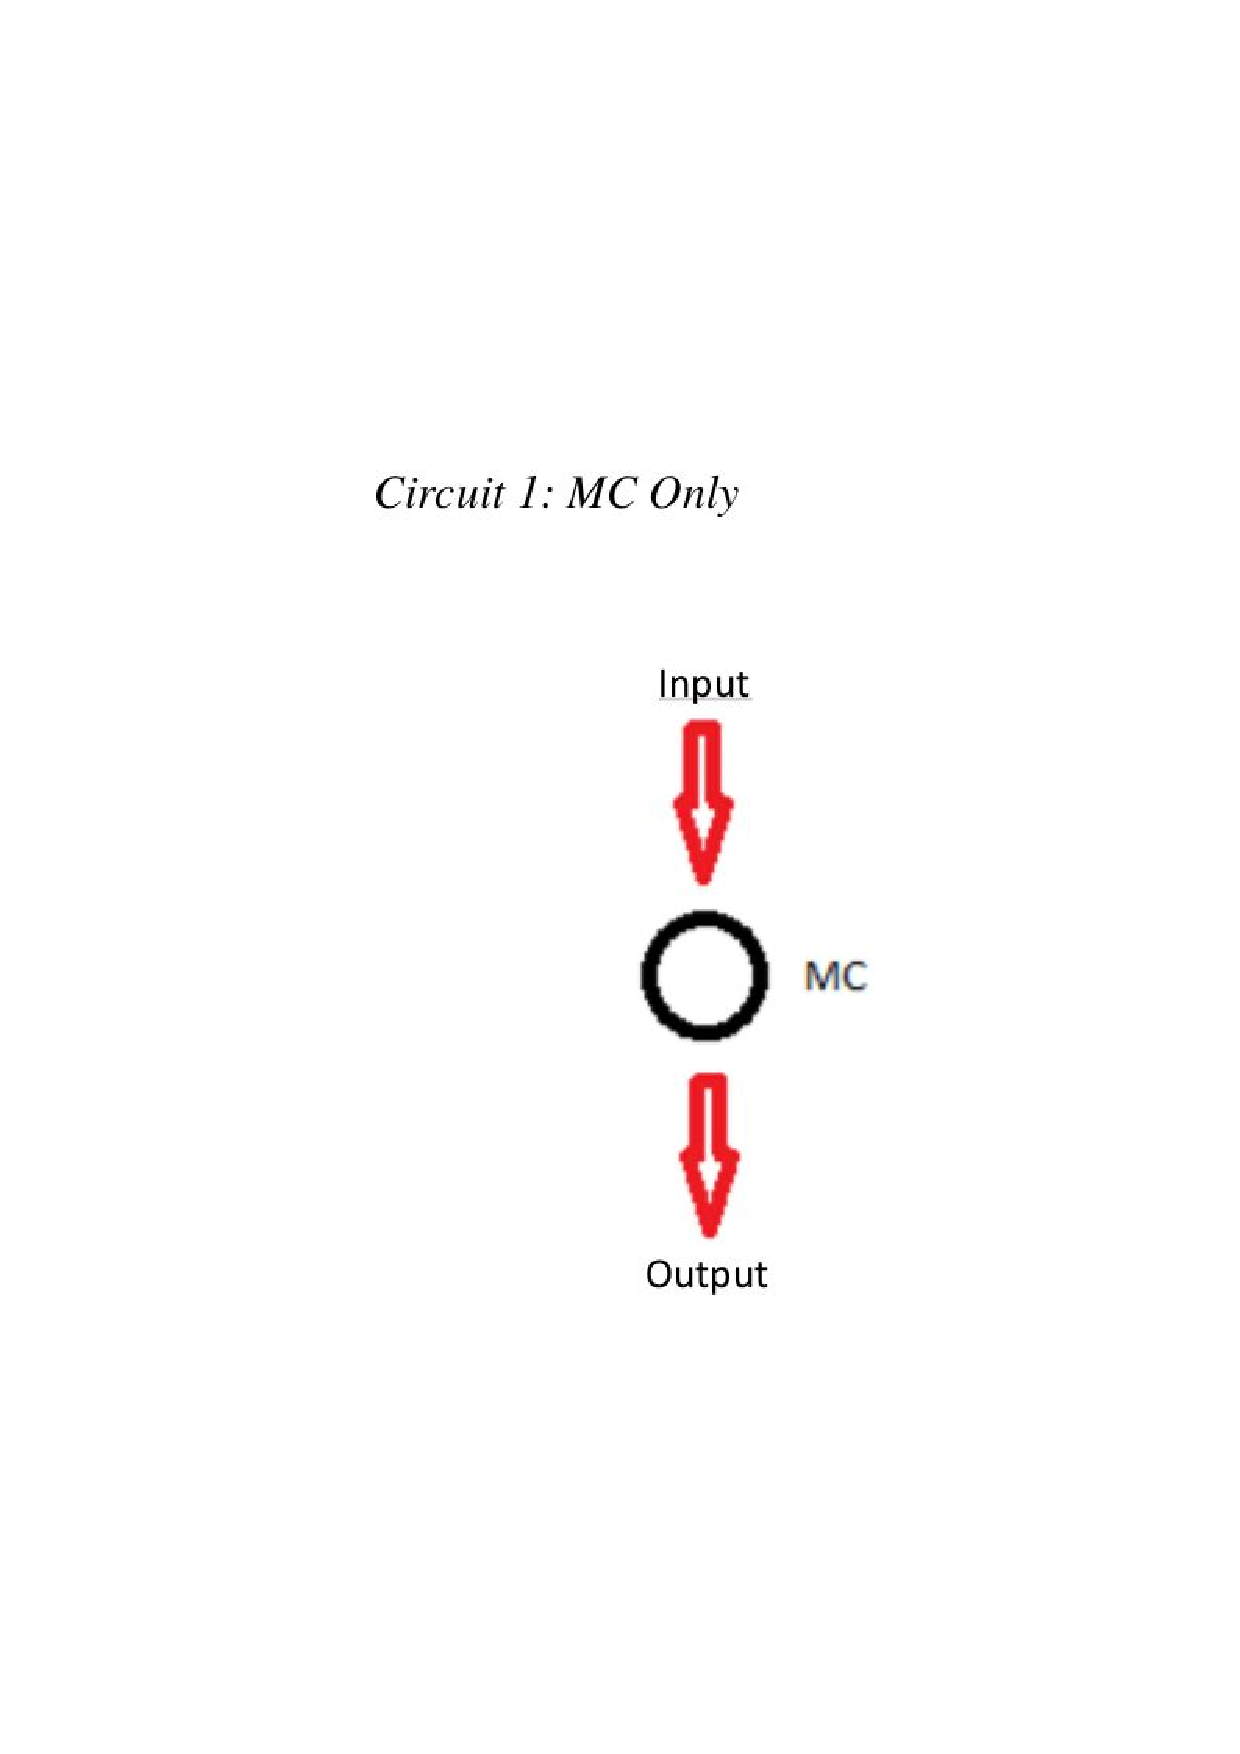
\includegraphics[trim={0 6cm 0 8cm},clip, scale=0.5]{Analysis-6-11-17/Circuit_1.pdf}
\caption{showing circuit 1. This focuses on the mitral cell only.}
\end{figure} 

\begin{figure}[!h]
\centering
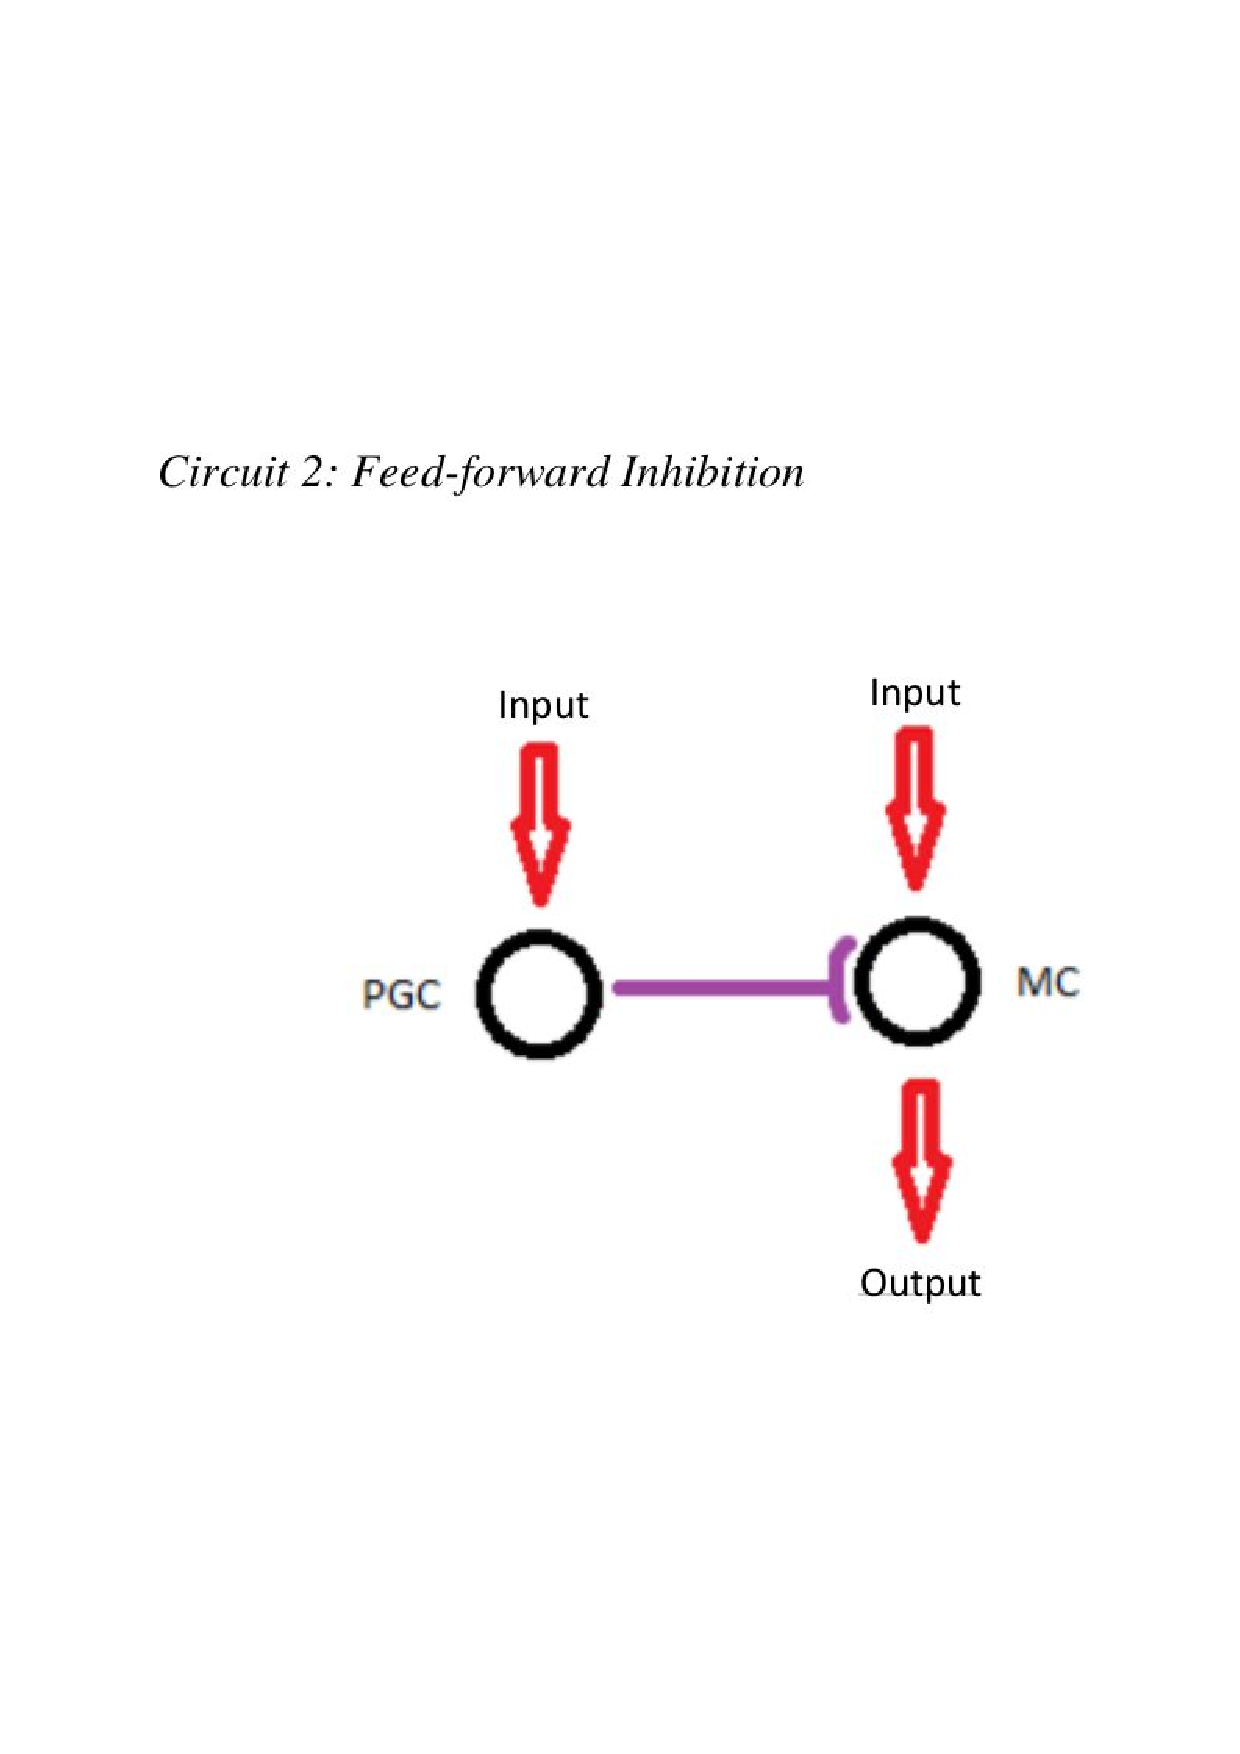
\includegraphics[trim={0 6cm 0 6cm},clip, scale=0.5]{Analysis-6-11-17/Circuit_2.pdf}
\caption{showing circuit 2. This focuses on the feed-forward inhibition.}
\end{figure} 
\newpage

\begin{figure}[!ht]
\centering
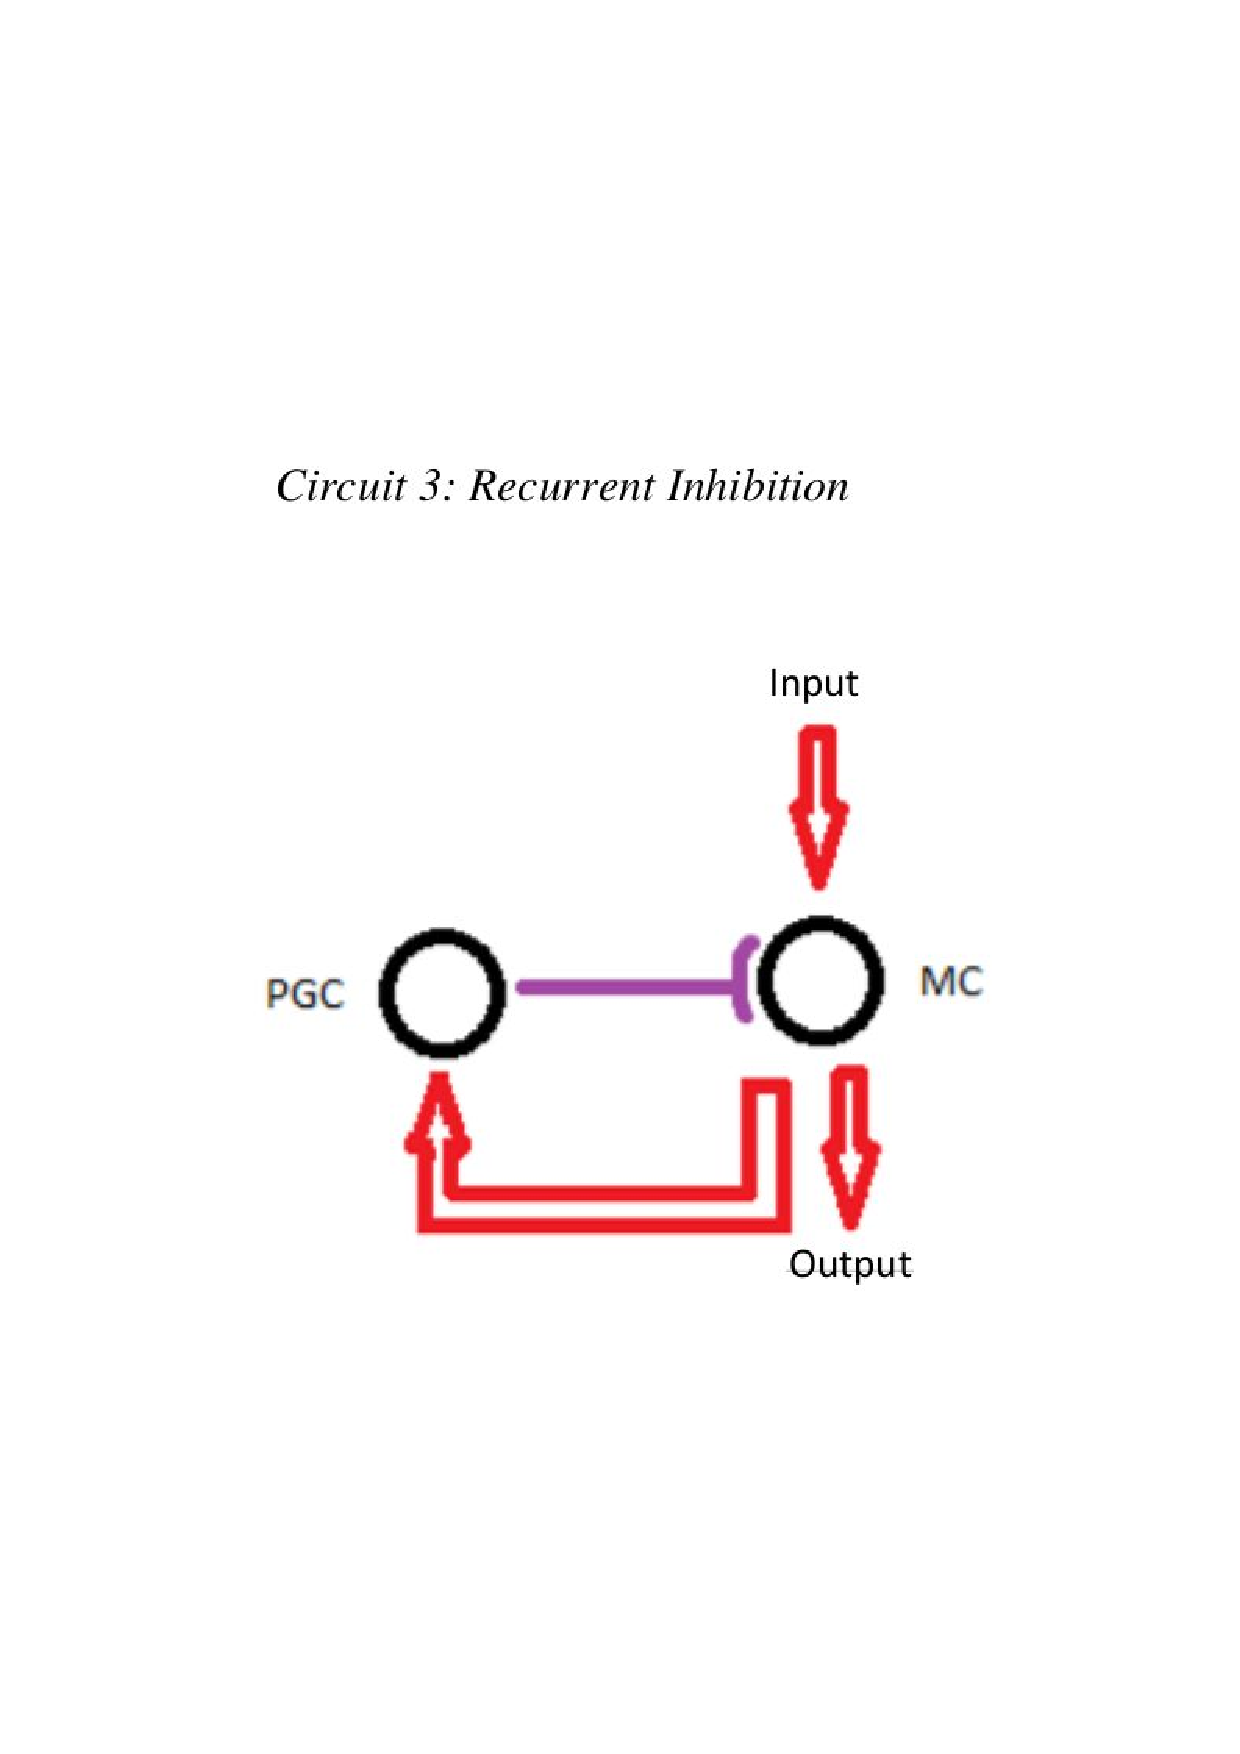
\includegraphics[trim={0 6cm 0 6cm},clip, scale=0.5]{Analysis-6-11-17/Circuit_3.pdf}
\caption{showing circuit 3. This focuses on the recurrent inhibition.}
\end{figure} 

Each aspect of the model was analysed individually, see figures 4, 5 and 6. Therefore, we can determine which mechanism is responsible for results found in figures 2 and 3.
\newpage

\begin{figure}[!ht]
\centering
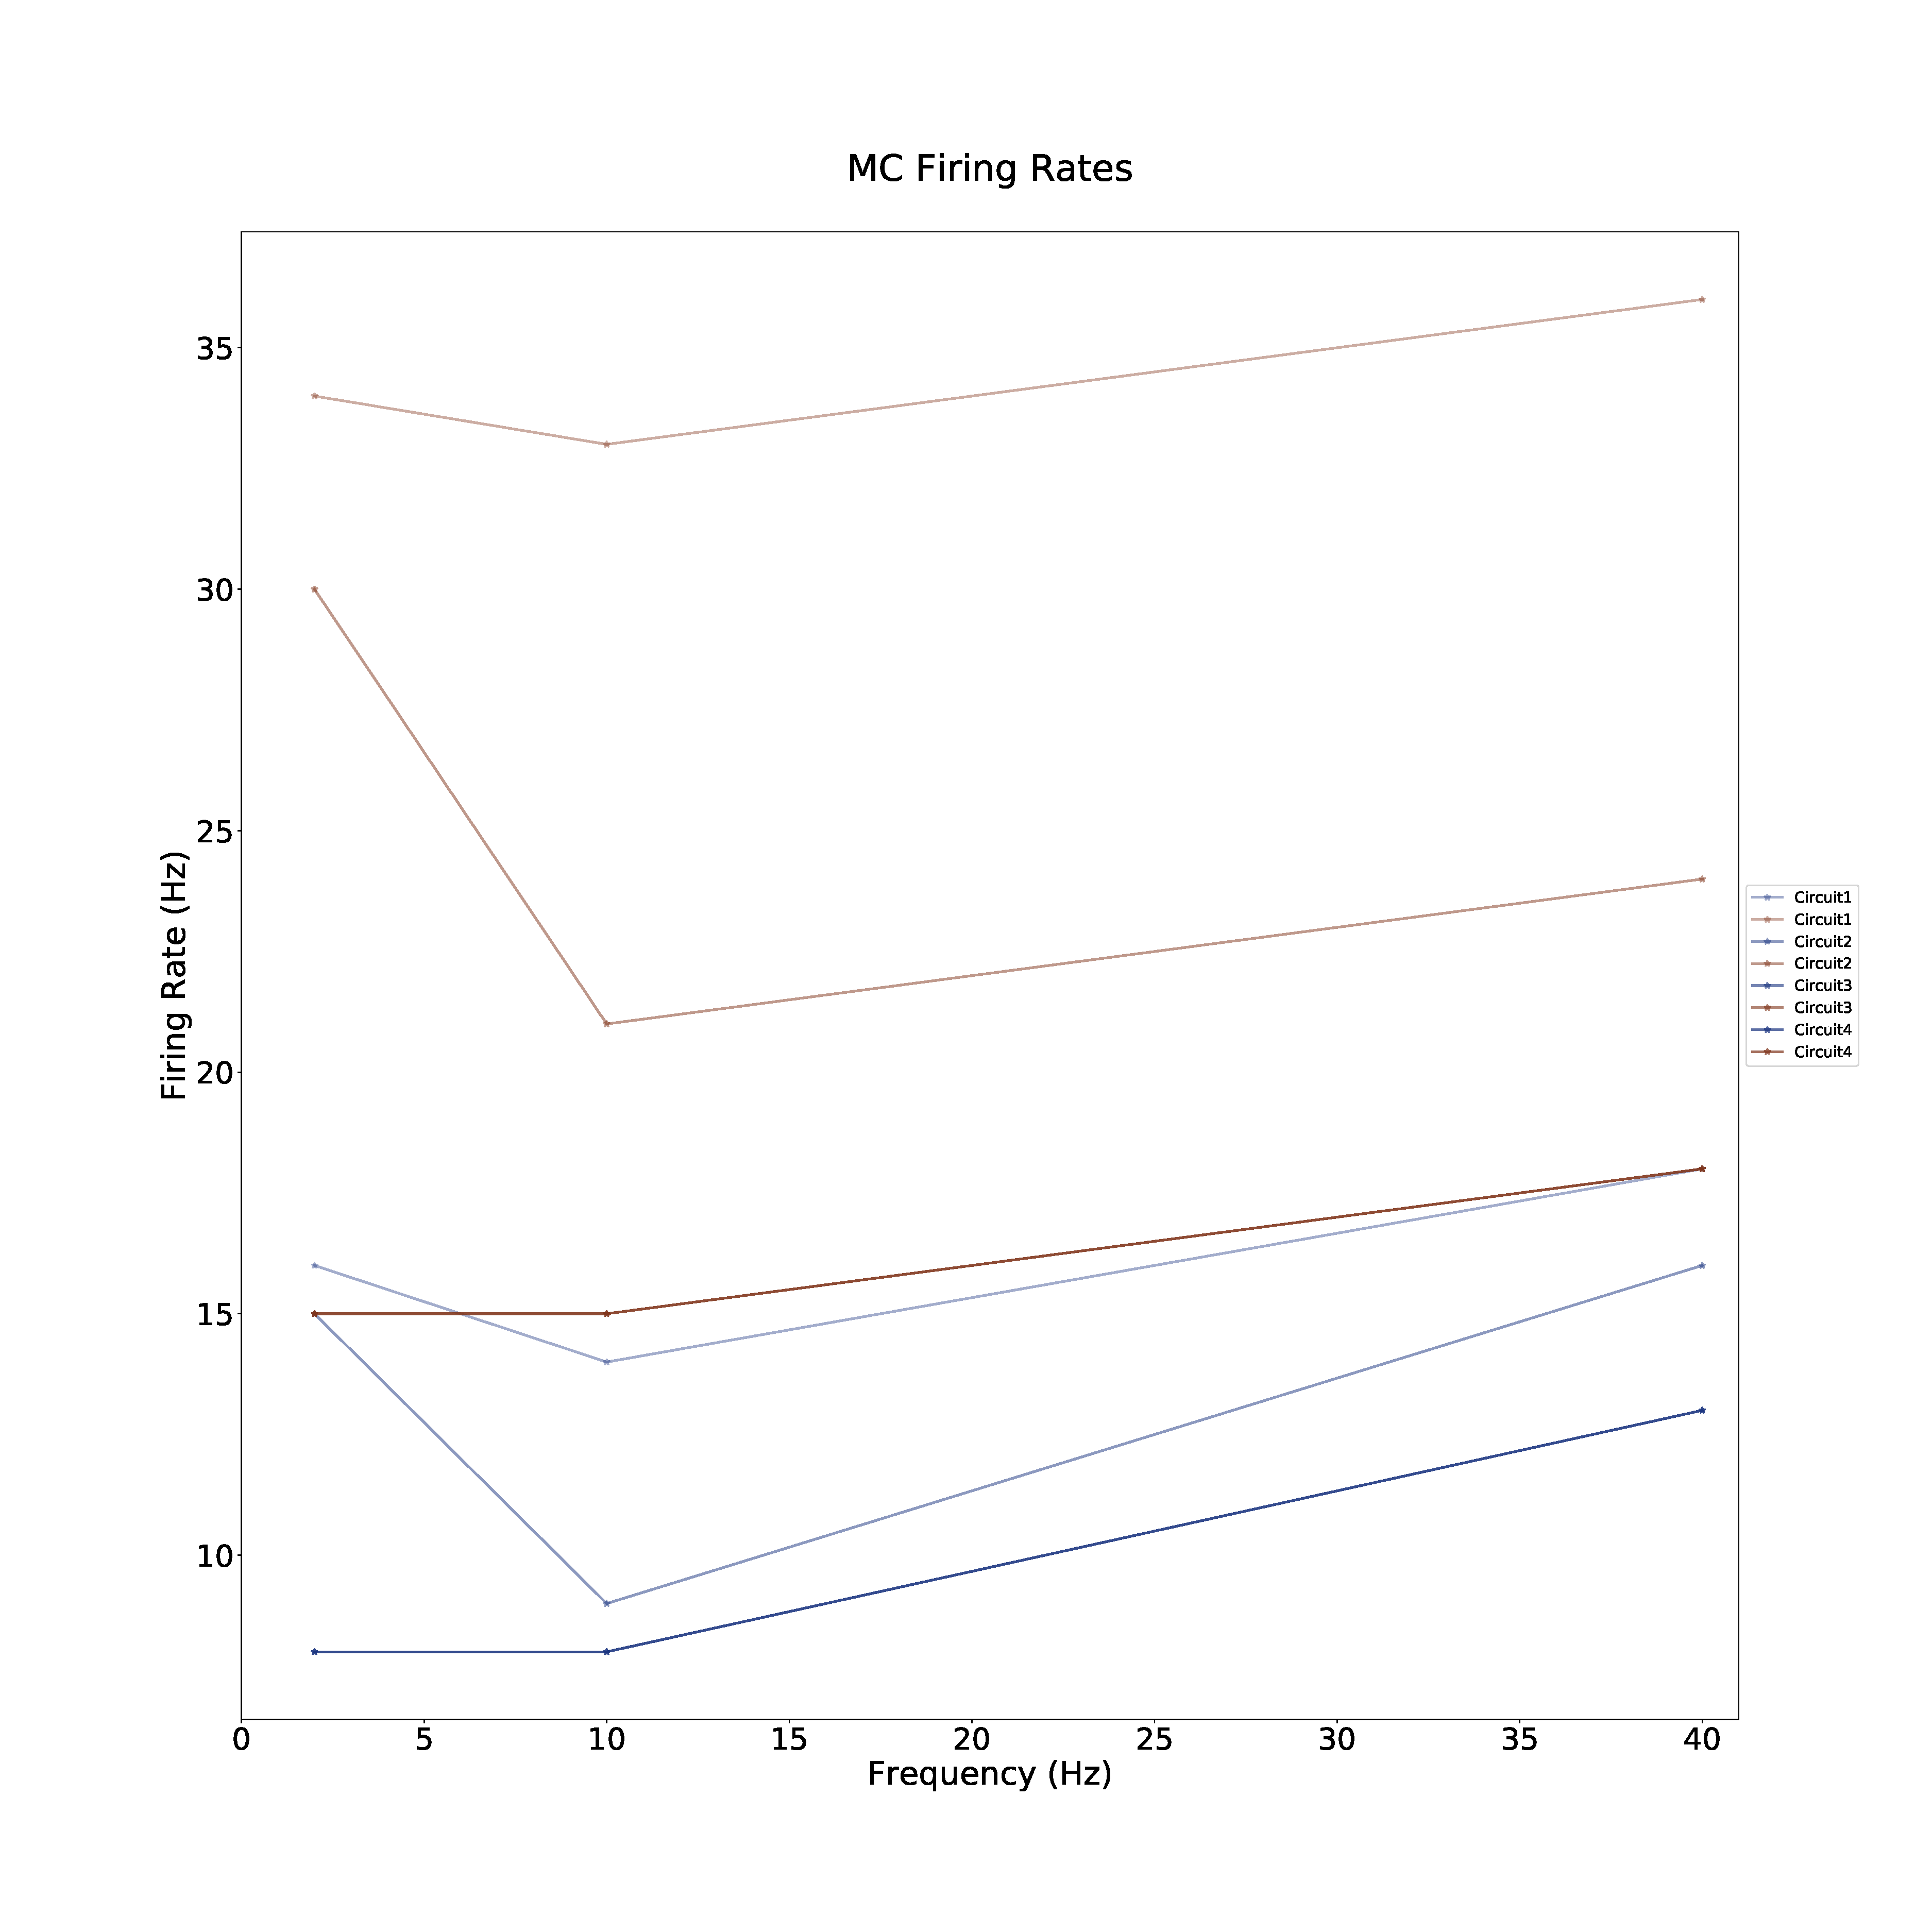
\includegraphics[scale=0.3]{Analysis-6-11-17/MC_firing_rate.pdf}
\caption{showing the mitral cell firing rates for all circuits.}
\end{figure} 

\begin{figure}[!ht]
\centering
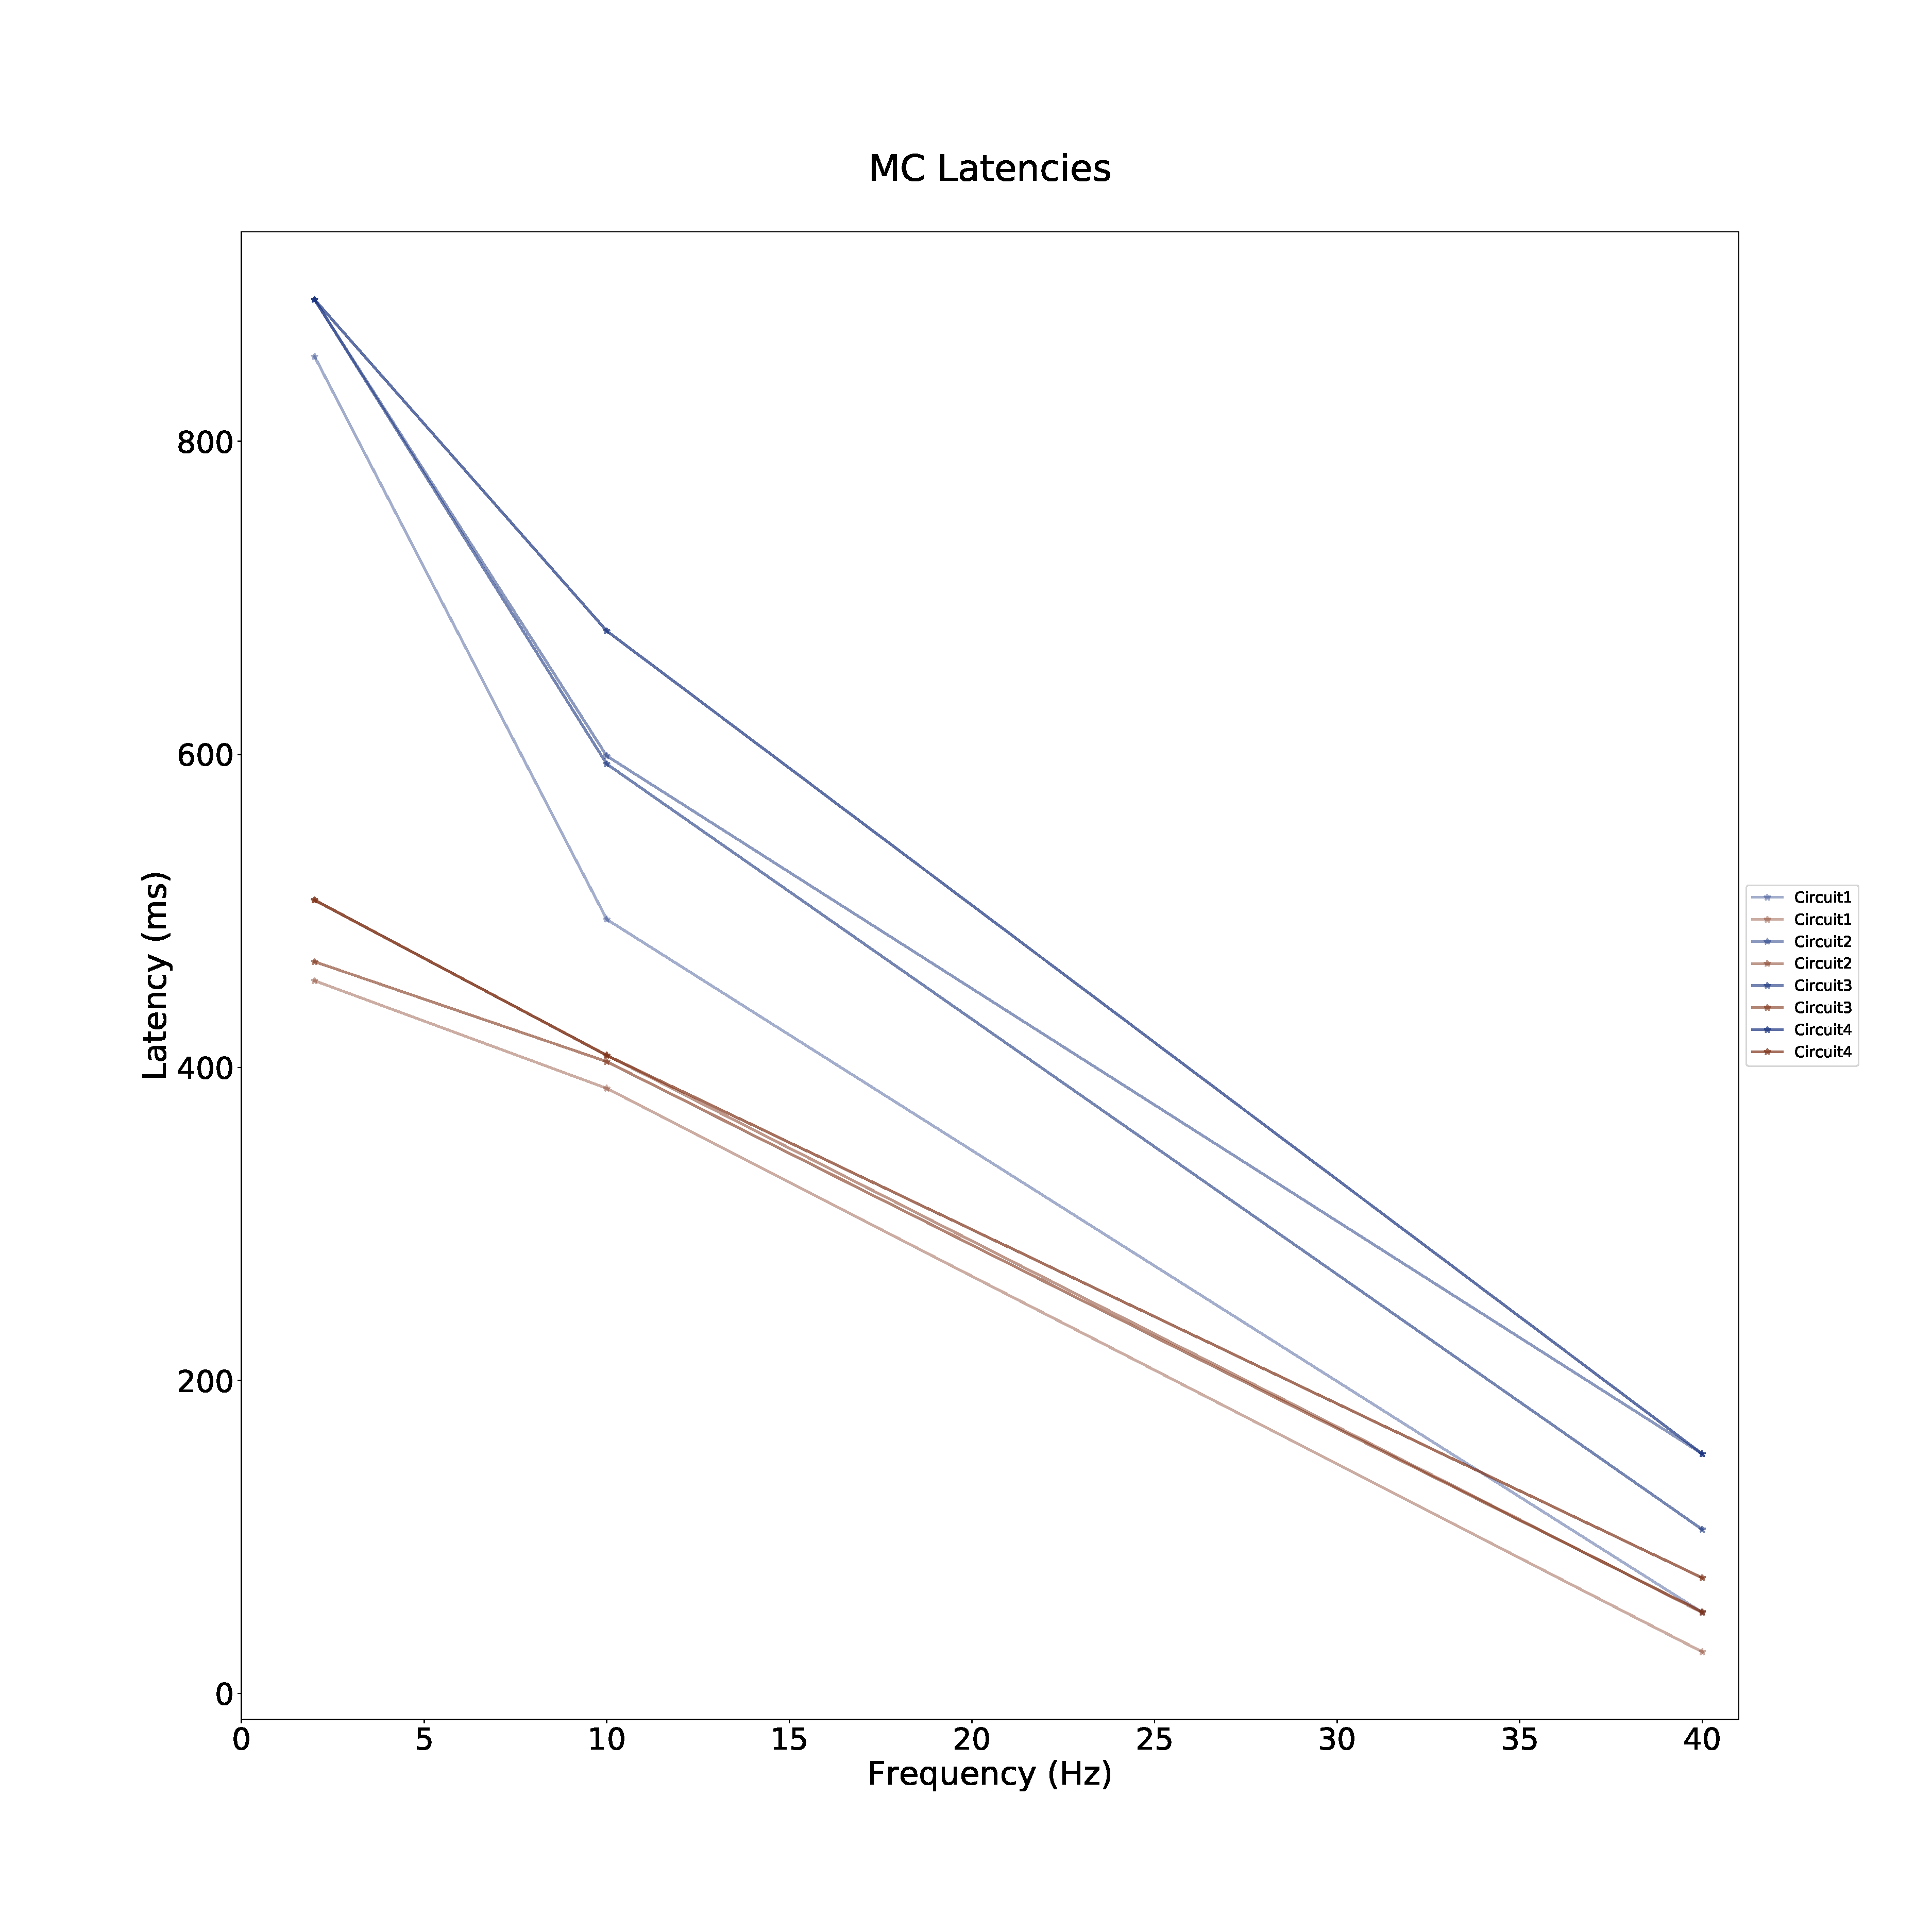
\includegraphics[scale=0.3]{Analysis-6-11-17/MC_latencies.pdf}
\caption{showing the mitral cell latencies for all circuits.}
\end{figure} 

\end{document}